\section{Informacinių technologijų taikymas sveikatos priežiūros įstaigose}
Eurostat duomenimis \cite{Eurostat}, 2017 metais, 19\% Europos sąjungos populiacijos sudarė 65 metų ir vyresni asmenys. Per paskutinius 10 metų, Lietuvoje 65 metų ir vyresnių asmenų skaičius padidėjo 2,7\%, o Europos sąjungoje - 2,4\%. Populiacijos senėjimo tendencija, pasak Eurostat, nežada keistis ir 2080 metais, 80 metų ir vyresni asmenys sudarys daugiau nei 12\% visos Europos sąjungos populiacjos. Pasak Pasaulio sveikatos organizacijos \cite{Organization2012}, per paskutinius 10 metų, Europos regione sveikatos priežiūros specialistų skaičius padidėjo 10\%, tačiau abejojama ar šis specialistų skaičiaus didėjimas bus pakankamas tam, kad padengtų senstančios populiacjos reikmes. Ši organizaciją kaip didžiausia problemą nurodo slaugytojų trukūmą. Kadangi Europos sąjungos populiacija sensta, specialistų nebeužtenka, vadinasi reikalingas sveikatos priežiūrios procesų efektyvumo didėjimas tam, kad padengtų populiacijus reikmes. Šių procesų efektyvumą galime didinti informacinių technologijų pagalba. Toliau šiame skyriuje apžvelgsime informacinių technologijų taikymą Lietuvos sveikatos priežiūros įstaigose.

\subsection{Gydymo įstaigų informacinės sistemos}
Gydymo įstaigų informacinė sistema, kitaip dar vadinama hospitalinė informacinė sistema (toliau - HIS), yra autonominė sveikatos priežiūros įstaigos sistema, kuri orentuojasi į šias veiklas - pacientų registravimas, priėmimas, išleidimas, perkėlimas, apmokestinimas ir kitos administracinės, finansinės ir medicininės funkcijos \cite{Sabooniha2012}. Tam, kad ši sistema išties gerintų sveikatos priežiūros procesų efektyvumą, reikalingas tinkamas duomenų paskirstymas tarp sveikatos priežiūros įstaigos skyrių, todėl šios sistemos pagrindinis uždavinys - apjungti visų skyrių informacines sistemas. Pati HIS nėra laikoma individualaus skyriaus informacine sistema \cite{JuliusGriskevicius}, ji priima klinikinius duomenis iš įstaigos skyrių informacinių sistemų ir juos saugo. Sveikatos priežiūros įstaigos specialistam prireikus pacientų klinikinių duomenų, HIS suteikia prieigą prie jų. Pagrindinės savybės apibūdinančios HIS \cite{JuliusGriskevicius}: 
\begin{enumerate}
    \item Informacijos apie pacientus duomenų bazės;
    \item Pacientų priėmimas ir lovų užimtumo kontrolė;
    \item Analizavimo įrankiai, kurie palengvina sprendimo priėmimą;
    \item Pacientų valdymas ir jų sveikatos įvertinimas;
\end{enumerate}


Tam, kad suprasti Lietuvos sveikatos priežiūros įstaigų naudojamų informacinių sistemų savybes ir funkcionalumus, autorius pasirinko išanalizuoti trijų sveikatos įstaigų HIS. Buvo pasirinkta Kauno regiono asmens sveikatos priežiūros įstaigų HIS (toliau - KRASPI), nes šią HIS naudoja Jonavos ligoninė ir Vilniaus universiteto ligoninės Žalgirio klinikos HIS (toliau - VULZK HIS). Šios dvi HIS buvo pasirinktos todėl, nes įstaigos, naudojančios šias HIS, buvo pasirinkos stacionaraus gydymo nagrinėjimui ankstesniame skyriuje. Taip pat buvo pasirinkta nagrinėti Vilniaus universiteto ligoninės Santaros klinikos HIS (toliau - VULSK HIS), nes tai yra viena iš didžiausių Lietuvos sveikatos priežiūros įstaigų. Išanalizavimus šių įstaigų HIS specifikacijas, buvo sudaryti palyginimo lentelė (žiūrėti 1 lentelę). 

\begin{table}[!ht]
    \centering
    \renewcommand{\arraystretch}{1.2}
    \begin{tabular}{| p{8em} | c | c | c |}\hline
        \backslashbox[8em]{Savybės}{Įstaigos}
        &\makebox[8em]{KRASPI}&\makebox[8em]{VULZK HIS}&\makebox[8em]{VULSK HIS}\\\hline
        Duomenų centralizuotas kaupimas &+ &+ &+\\\hline
        Pacientų valdymas &+ &+ &+\\\hline
        Duomenų analizavimo įrankiai &- &- &+\\\hline
        Pacientų sveikatos vertinimas &+ &+ &+\\\hline
        Finansinių dokumentų paruošimas &- &+ &+\\\hline
        Lovų užimtumo kontrolė &+ &+ &+\\\hline
    \end{tabular}
    \caption{Sveikatos priežiūros įstaigų informacinių sistemų palyginimas}
    \label{HIS}
\end{table}

Atlikus palyginimą, buvo išsiaiškinta, kad visos nagrinėjamos HIS pasižymi panašiomis savybės ir sprendžia bendras problemas, tačiau tiek Jonavos ligoninės naudojamame HIS, tiek Žalgirio klinikos HIS, trūksta duomenų analizavimo įrankių, taip pat KRASPI nėra finansinių dokumentų paruošimo funkcionalumo.

% &\makebox[8em]{Kauno regiono asmens sveikatos priežiūros įstaigų}&\makebox[8em]{Vilniaus universiteto ligonin4s Santariškių klinikos}&\makebox[8em]{Vilniaus universiteto ligoninės Žalgirio klinika}\\\hline

\subsection{Elektroninė sveikatos paslaugų ir bendradarbiavimo infrastruktūros informacinė sistema}
\subsubsection{Sistemos apžvalga}
Ankstesniame poskyryje apžvelgėme gydymo įstaigų informacines sistemas, tačiau pacientams ne visada sveikatos priežiūros paslaugos teikiamos vienoje gydymo įstaigoje. Pacientus gydymo įstaigą, iškyla problema - klinikinių paciento duomenų perkėlimas. Šia problemą išsprendžia visos Lietuvos mąstu naudojama elektroninė sveikatos paslaugų ir bendradarbiavimo infrastruktūros informacinė sistema (toliau - ESPBI IS). ESPBI IS yra apibrėžiama kaip priemonių visuma, kuri skirta centralizuotai kaupti, formuoti ir naudoti pacientų sveikatos istorijas \cite{ESPBINuostatos}. Šios sistemos dėka, įstaigos, kurios turi prieigos teises, gali tarpusavyje keistis pacientų informacija. Lietuvoje ESPBI IS buvo diegiama 3 etapais, diegimo datos pradžia - 2007 metai, o pabaiga - 2015 metai \cite{Ministras2015}. Kadangi ESPBI IS yra didelės apimties projektas, kuris truko beveik dešimtmetį, dalykinės srities reikalavimai buvo klasifikuojamas ir kuriami mažesni projektai šiems reikalavimams įgyvendinti. Pagrindiniai ESPBI IS projektai \cite{Specifikacija}:
\begin{enumerate}
    \item \textbf{Elektroninės sveikatos paslaugų ir bendradarbiavimo infrastruktūra}.
    
    Šio projekto metu sukurtos sistemos pagrindinis funkcionalumas:
    \begin{enumerate}
        \item Pacientų elektroninio sveikatos įrašo tvarkymas;
        \item Paciento registravimasis arba išsiregistravimasis iš sveiktos priežiūros įstaigoje;
        \item Sąveika tarp skirtingų sveikatos priežiūros įstaigų informacinių sistemų;
        \item Aktualių paciento duomenų teikimas ir gavimas;
        \item Finansinių ataskaitų tvarkymas;
        \item Elektroninės tapatybas nustatymas.
    \end{enumerate}
    \item \textbf{Elektroninis receptas}. 
    
    Šio projekto metu sukurtos sistemos pagrindinis funkcionalumas:
    \begin{enumerate}
        \item Elektroninių receptų ar kompensuojamų medicininės pagalbos priemonių išrašymas;
        \item Centralizuotas išrašytų receptų registravimas;
        \item Elektroninių receptų informacijos pateikimas pacientams.
    \end{enumerate}

    \item \textbf{MedVAIS}.
    
    Šio projekto metu sukurtos sistemos pagrindinis funkcionalumas:
    \begin{enumerate}
        \item Sveikatos priežiūros įstaigų sukurtų medicinių vaizdų tvarkymas medicininių vaizdu tvarkymo posistemėje;
        \item Medicininių vaizdų pateikimas pacientams;
        \item Medicinių vaizdų pateikimas gydytojams;
        \item Nuasmeninto medicininio vaizdo pateikimas;
    \end{enumerate}
\end{enumerate}

Kadangi autoriaus projektuojama sistema nėra susijusi nei su medicininiais vaizdai, nei su elektroniniais receptais, tolimesniame nagrinėjime autorius didesnį dėmesį skiria pirmojo projekto analizavimui, o sekantiems dviem projektam dėmesys skiriamas mažesnis.


ESPBI IS paskirtis yra išskiriama į paciento ir sveikatinimo įstaigų atžvilgius \cite{Ltrsam}. Paciento atžvilgiu ESPBI IS paskirtis yra:
\begin{itemize}
    \item Gerinti sveikatingumo paslaugų prieinamumą ir testinumą;
    \item Turėti prieigą prie sveikatą apibūdinančių dokumentų;
    \item Plėtoti elektroninės sveikatos paslaugos, užtrikinant, kad pacientai būtų tinkamai informuojami apie teikiamas paslaugas.
\end{itemize}


Sveikatinimo įstaigų atžvilgiu ESPBI IS paskirtis yra:
\begin{itemize}
    \item Pašalinti paciento duomenų dubliavimą;
    \item Užtikrinant administracinio darbo efektyvumą;
    \item Plėtoti elektroninės sveikatos paslaugos, užtrikinant, kad įstaigos bendradarbiautų ir gautų aktualią paciento informaciją;
    \item Užtikrant elektroninės sveikatos paslaugų efektyvumą;
    \item Užtikrinti priegą prie centralizuotos informacijos.
\end{itemize}

Apibendrinant išvardintas šios sistemos paskirtis, galima teigti, kad siekiama, jog pacientas turėtų galimybę peržiūrėti savo sveikatos istoriją elektroniniu būdų, o įstaigos, efektyviai keistūsi paciento informacija ir ją naudotų tam, kad paslaugų kokybė gerėtų.

\subsubsection{Sistemos architektūra}

Pagal ESPBI IS specifikaciją \cite{Specifikacija} autorius parengė abstrakčią ESPBI IS architektūros diagramą (žiūrėti 1 pav.). 

\begin{figure}[H]
    \centering
    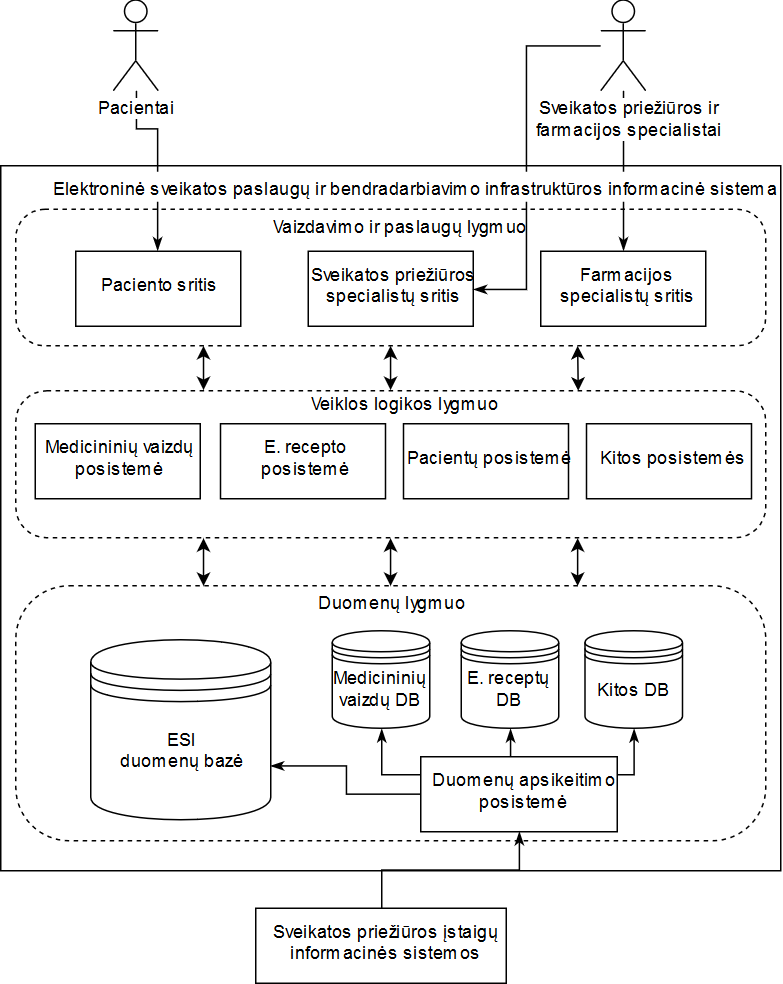
\includegraphics[scale=0.45]{images/ESPBI}
    \caption{Elektroninės sveikatos paslaugų ir bendradarbiavimo infrastruktūros informacinės sistemos achitektūra} 
\end{figure}
% perpiesti, reikia prideti esi posisteme


Pagal parengtos architektūros diagramą matome, kad architektūra yra 3 lygmenų - vaizdavimo ir paslaugų, veiklos logikos ir duomenų lygmens. Išnagrinėkime šiuos tris lygmenis: 

\begin{itemize}
    \item \textbf{Vaizdavimo ir paslaugų lygmuo}. Šį lygmenį sudaro elektroninės sveikatos portalo posistemė. Šio portalo paskitis - medicinių paslaugų iniciavimas, šių paslaugų informavimas, jų vykdymo stebėjimas ir suteiktų paslaugų rezultatų pateikimas.
    informavimui/komunikavimui ir rezultatų pateikimui \cite{Specifikacija}. Šios sistemos naudotojai yra identifikuojami elektroniniu parašu. Prisijungusiam naudotojui yra pateikiamas turinys pagal identifikavimo metu suteiktas prieigas. Elektroninė sveikatos portalo posistemė susideda iš 4 sričių:
    \begin{enumerate}
        \item Viešai prieinama sritis. Šioje elektroninės sveikatos portalo srityje yra pateikiama visiem prienama informacija. Tam, kad naudotojas pasiektų šią informaciją, jam savo tapatybės identifikuoti nereikia;
        \item Pacientų sritis. Šioje elektroninės sveikatos portalo srityje yra pateikiama pacieto gautų paslaugų informacija, rezultatai, išrašytų elektroninių receptų duomenys ir kt;
        \item Sveikatos priežiūros specialistų sritis. Šioje elektroninės sveikatos portalo srityje yra sveikatos priežiūros specialistai gali pildyti elektroninės sveikatos priežiūros formas, tvarkyti pacientų duomenis, gauti aktualus paciento klinikinius duomenis, medicininius vaizdus, taip pat specialistas, turintis reikiamą prieiga, gali išrašyti pacientui elektroninė receptą, pratęsti jo galiojimo terminą,
        \item Farmacijos specialistų sritis; Ši elektroninės sveikatos portalo sritis yra skirta farmacijos specialistam. Ji leidžia naudotojam gauti informaciją apie išrašyti elektroninį receptą ir patvirtinti vaistų ar medicinių pagalbos priemonių išdavimo faktą.
    \end{enumerate}
    \item \textbf{Veiklos logikos lygmuo}. Šis lygmuo yra tarpinis tarp vaizdavimo ir duomenų lygmenų.  Veiklos logikos lygmens pagrindinė paskirtis yra priimti sisteminius pranešimus, juos apdoroti, sugeneruoti reikiamą informaciją ir šią informaciją pateikti vaizdavimo ir paslaugų lygmeniui \cite{Specifikacija}. Taip pat šis lygmuo priima duomenis iš elektroninio sveikatos portalo, šiuos duomenis apdoroja ir perduoda į duomenų lygmenį. Apibendrinant šio lygmens paskirtį - tai centrinis funkcionalumų lygmuo, kuris apdoroja ir pateikia reikalingus duomenis apie pacientą, elektroninius receptus, medicininius vaizdus ir kt. Šį lygmenį sudaro 11 posistemių, tačiau pagrindinės yra: 
    \begin{enumerate}
        \item Pacientų posistemė;
        \item Medicinių vaizdų posistemė;
        \item Elektroninio recepto posistemė;
        \item Duomenų analizės, ataskaitų formavimo ir informavimo posistemė;
        \item Elektroninio sveikatos įrašo posistemė.
    \end{enumerate}
    \item \textbf{Duomenų lygmuo}. Duomenų lygmuo susideda iš 2 komponentų - informacinės struktūros ir duomenų mainų posistemės. Apžvelgsime šiuos komponentus:
    \begin{itemize}
        \item Informacinė struktūra. Šis komponentas atsakingas už ESPBI IS informacijos tvarkymą, saugojimą, apdorojimą ir teikimą. Pagrindinis informacinės struktūros komponentas yra ESI duomenų bazė, tačiau informacinė struktūrą sudaro ir daugiau papildomų duomenų bazių \cite{Specifikacija}, iš viso yra 10 duomenų bazių, kurios saugo informaciją apie sveikatos priežiūros paslaugų teikimą. ESI duomenų bazėje saugomi pacientų elektroniniai sveikatos įrašai, kurie yra suvedami paslaugų ir vaizdavimo lygmenyje arba gaunami iš sveikatos priežiūros įstaigų informacinių sistemų. Kiekvienas įrašas yra susiejimas su identifikatoriumi, kuris yra suteikiamas Objektų ID katalogo. Objektų ID katalogas suteiktą identifikatorių susieja su paciento įrašu, specialistu, kuris pateikė paciento įraša, ir sveikatos priežiūros įstaiga. ESI duomenų bazės tvarkomi dokumentai \cite{Specifikacija} - ypatingieji pacientų duomenys, ESI suformavusių sveikatinimo specialistų duomenys, ESI pateikusių sveikatinimo įstaigų duomenys;
        \item Duomenų mainų posistemė. Šis komponentas atsakingas už duomenų priėmimą bei atidavimą sveikatos priežiūros įstaigų informacinėms sistemos bei kitoms suinteresuotų trečiųjų šalių informacinėms sistemos. Ši posistemė yra kertinis komponentas, kuris realizuoja techninio interoperabilumo princpus elektroninės sveikatos sistemoje \cite{Specifikacija}. Duomenų mainų posistemės pagrindinė paskirtis - valdyti duomenų mainus tarp sveikatos priežiūros įstaigų ir užtikrinti duomenų gavimą bei teikimą tokioms įstaigom kaip SODRA, SVEIDRA, VAPRIS ir kitomis valstybinėms institucijom. Visi duomenų mainai tarp ESPBI IS ir kitų informacinių sistemų vyksta per šią posistemę.
    \end{itemize}
\end{itemize}

\subsubsection{Septinto lygio sveikatos standartas}
Ankstesniuose poskyriuose apžvelgėme Lietuvos sveikatos priežiūros įstaigų naudojamas informacines sistemas, tačiau Lietuva nėra išskirtinė šioje srityje ir kitos Europos sąjungos valstybės taip pat diegia bei naudoja tokio pat pobūdžio informacines sistemas, šių sistemų diegimo bei naudojimo būsena yra aprašyta Europos Komisijos \cite{EuroposKomisija}. Europos parlamento priimtose direktyvose \cite{EuroposParlamentas} yra nurodoma, jog valstybės turi tarpusavyje dalintis pacientų sveikatos įrašais, t.y. pacientui apsilankius svetimos valstybės sveikatos priežiūros įstaigoje, ši įstaiga galėtų gauti paciento duomenis iš jo gimtosios valstybės. Kadangi siekiama pacientų duomenų keitimosi ne tik regioniniu mąstu, bet ir tarpvalstybiniu, vadinasi visos tarpusavyje komunikuojančios informacinės sistemos turi vadovautis bendru tarptautiniu standartu, kuris aprašytų pacientų duomenų apsikeitimo procesą. Toks pacientų duomenų apsikeitimo standartas yra Septintojo lygio sveikatos standartas (angl. \textit{Health Level Seven International})(toliau - HL7). HL7 standartas, kurio pirmoji versija buvo sukurta 1987 metais, yra patvirtintas Amerikos nacionalinio standartų instituto, šis standartas apibrėžiantis elektroninių sveikatos įrašų paiešką, dalijimasi, integraciją ir apsikeitimą \cite{HL72009}. HL7 nusako kaip elektroniniais sveikatos įrašais įstaigos keičiasi ir kokiu duomenų formatu šie įrašai yra suformuoti. HL7 yra apibrėžęs 2 duomenų formatus - v2 ir v3, taip pat egzistuoja ir FHIR standartas, kuris apjungia labiausiai pasiteisinusis HL7 v2 ir v3 standartų aspektus. ESPBI IS specifikacijoje yra \cite{Specifikacija} nurodoma, jog duomenų apsikeitimui yra naudojamas HL7 v3 arba FHIR standartai, tačiau naujesnėje literatūroje \cite{Registrucentras} yra nurodomas tik FHIR. FHIR standartas apibrėžia netik duomenų formavimą, bet ir pateikia REST architektūra pagrįstą interfeisą, kuris nurodo
% paaiskint interfeisa ir resta, crud
duomenų operacijoms reikalingus CRUD metodus.


% issiaiskinti del ruklos, kam ji priklauso ( Jei priklauso kazkam is saraso, galim prideti saltini prie hospitalisation.tex)
% neiasku del duomenu baziu, lape raso, kad ji viena yra, o realiai ju daug